% General Configs

\documentclass[10pt, compress]{beamer}

%---------------------------------------------------------
%---------------------------------------------------------
\usepackage[alf]{abntex2cite}
\usepackage[utf8]{inputenc}
\usepackage[portuguese]{babel}
\usepackage{graphicx}			% Inclusão de gráficos
\usepackage{float} 				% Fixa tabelas e figuras no local exato
\usepackage{physics}
\usepackage{bbold}
\usepackage{subcaption}
\usepackage{mathtools}
\usepackage{xcolor}
\usepackage{appendixnumberbeamer}
\usepackage{svg}
\usepackage{multirow}
 \usepackage{amsmath} 
 \usepackage[table]{xcolor}
 \usepackage{xcolor}
 \usepackage{pdfpages}
 
%------------------Tikz
\usepackage{tikz}
\usetikzlibrary{shapes,positioning,calc,quotes}
\tikzstyle{subrotina} = [rectangle, draw,text centered, minimum width=5em, inner sep=5pt]
\tikzstyle{funcao} = [rounded rectangle, draw, text centered, minimum width=7em, inner sep=5pt]
\tikzstyle{random} = [rectangle, text centered, inner sep=5pt, minimum width=5em]
\tikzstyle{loop} = [rectangle, draw, align=left]
\tikzstyle{fluxo} = [draw, thick, -latex]
\tikzstyle{meiofluxo} = [draw, -]
\tikzstyle{chamada} = [draw, dashed, <->]
\usepackage{tikzfill}
\usetikzlibrary{arrows.meta}
\usepackage{hyperref}
\usetikzlibrary{calc}
\usetikzlibrary{plotmarks}
\usepackage{pgfplots}
\usepackage{float}
\usepackage{csquotes}
\usepackage{mathrsfs}
\usetikzlibrary{arrows}
\usepgfplotslibrary{statistics}
\usepgfplotslibrary{fillbetween}
\usetikzlibrary{patterns}% <- added
\pgfplotsset{width=6cm,compat=1.9}

\usepackage{physics}
\usetikzlibrary{calc}
\tikzset{>=latex} % for LaTeX arrow head
\usepackage{xcolor}
\colorlet{veccol}{green!45!black}
\colorlet{myred}{red!90!black}
\colorlet{myblue}{blue!90!black}
\colorlet{mypurple}{blue!50!red!80!black!80}
\tikzstyle{vector}=[->,thin,veccol]
\usetikzlibrary{arrows.meta}
\tikzstyle{thin arrow}=[dashed,thin,-{Latex[length=4,width=3]}]
%-----------------------

%------------------------------------------------------------
% Configure Theme like things

\usetheme{Madrid}
\usefonttheme{structuresmallcapsserif}
\useoutertheme{miniframes} % Alternatively: miniframes, infolines, split
\useinnertheme{circles}
\setbeamercovered{transparent}

\definecolor{UBCblue}{rgb}{0.04706, 0.13725, 0.26667} % UBC Blue (primary)
\usecolortheme[named=UBCblue]{structure}

%------------ proportions in footer
\makeatletter
\setbeamertemplate{footline}
{
	\leavevmode%
	\hbox{%
		\begin{beamercolorbox}[wd=.333333\paperwidth,ht=2.25ex,dp=1ex,center]{author in head/foot}%
			\usebeamerfont{author in head/foot}\insertshortauthor\expandafter\beamer@ifempty\expandafter{\beamer@shortinstitute}{}{~~(\insertshortinstitute)}
		\end{beamercolorbox}%
		\begin{beamercolorbox}[wd=.4\paperwidth,ht=2.25ex,dp=1ex,center]{title in head/foot}%
			\usebeamerfont{title in head/foot}\insertshorttitle
		\end{beamercolorbox}%
		\begin{beamercolorbox}[wd=.266666\paperwidth,ht=2.25ex,dp=1ex,right]{date in head/foot}%
			\usebeamerfont{date in head/foot}\insertshortdate{}\hspace*{2em}
			\insertframenumber{} / \inserttotalframenumber\hspace*{2ex} 
	\end{beamercolorbox}}%
	\vskip0pt%
}
\makeatother
%------------- background image title page
\addtobeamertemplate{title page}{
	\begin{tikzpicture}[remember picture,overlay]
		\node[anchor=south west,inner sep=0pt] at (-4,-2.2)
		{
			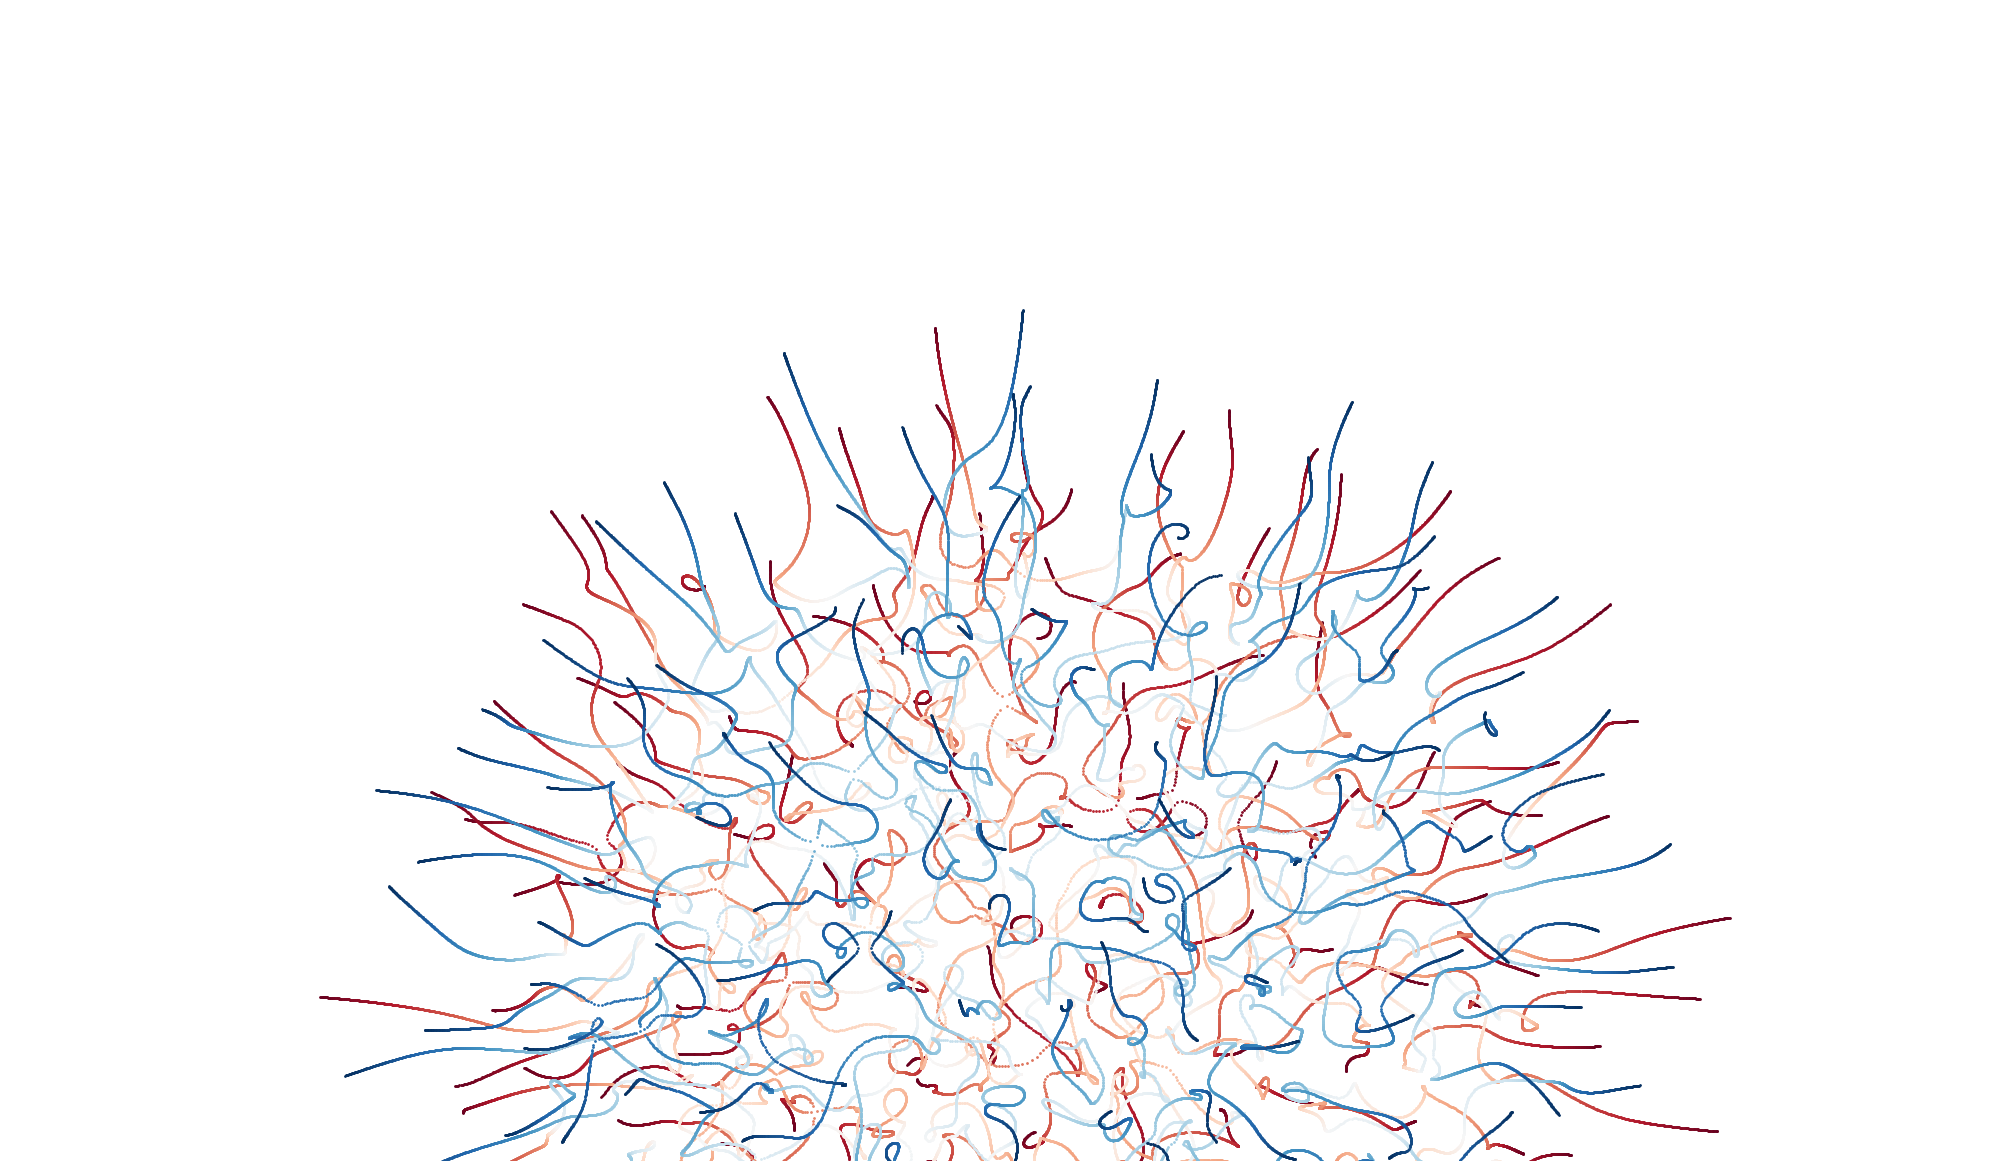
\includegraphics[width=1.5\paperwidth]{./media/aesthetics/croppedCircle.png}
		};
	\end{tikzpicture}
}{}
%------------

%TOC
\setbeamertemplate{section in toc}[sections numbered]
\setbeamertemplate{subsection in toc}[subsections numbered]
\setbeamerfont{subsection in toc}{size=\small, shape=\itshape}

%Templetae
\setbeamertemplate{navigation symbols}{}
\setbeamertemplate{note page}[compress]

%------------------------------------------------------------
%This block of code defines the information to appear in the
%Title page
\title[Asymptotics of Partition Functions of Coulomb Gases] %optional
{Asymptotics of Partition Functions of Coulomb Gases}

\subtitle{}

\author[João V. A. Pimenta] % (optional)
{João V. A. Pimenta\inst{1}}

\institute[ICMC] % (optional)
{
	\inst{1}%
	Insitituto de Ciências Matemáticas e de Computação - ICMC\\
	Universidade de São Paulo - USP
}

\date[Masters 2026] % (optional)
{Dissertation's defence for the degree of Master of Sciences in Mathematics. \\
Supervisor: Guilherme Silva}

\titlegraphic{
\includegraphics[height=1cm]{media/aesthetics/icmclogonb}}

%End of title page configuration block
%------------------------------------------------------------

%------------------------------------------------------------
%The next block of commands puts the table of contents at the 
%beginning of each section and highlights the current section:

\AtBeginSection[]{
	\begin{frame}
		\vfill
		\centering
		\includesvg[inkscapelatex=true, width=0.3\textwidth]{\secimage}
%		\begin{tikzpicture}
%		\begin{axis}[axis line style={opacity=0}, ticks=none,
%			xmin=-1.5, xmax=1.5,
%			ymin=-1.5, ymax=1.5,
%			xticklabel=\empty,
%			yticklabel=\empty,
%			xlabel={t = 0},
%			ylabel={a = 2},
%			xticklabel pos=top,
%			scatter/classes={%
%				a={ mark size=0.5pt}}
%			]
%			\addplot[skip coords between index={50}{500}, opacity=1, scatter, mark=x, black, only marks] table [col sep=comma] {\secimage};
%			\addplot[opacity=0.05, scatter, mark=*,draw opacity=0,black, only marks] table [col sep=comma] {\secimage};
%		\end{axis}
%		\end{tikzpicture}
		\begin{beamercolorbox}[sep=8pt,center,shadow=true,rounded=true]{title}
			\usebeamerfont{title}\insertsectionhead\par%
		\end{beamercolorbox}
		\vfill 
	\end{frame}
}

%------------------------------------------------------------
\definecolor{titleideablock}{HTML}{014508}
\definecolor{historycolor}{HTML}{b36630}
\definecolor{preamblecolor}{HTML}{d97836}



\newenvironment{ideablock}[1]{%
	\setbeamercolor{block title}{bg=titleideablock}
	\begin{block}{#1}}{\end{block}}

\newenvironment{history}[1]{%
	\setbeamercolor{block title}{bg=historycolor}
	\begin{block}{#1}}{\end{block}}
%------------------------------------------------------------

%------------------------------------------------------------
% math when ellipsis
%------------------------------------------------------------
\newcommand{\many}[2]{$#1_1, #1_2, \dots, #1_#2$}
\newcommand{\cmany}[3]{$#1_1 #3 #1_2 #3 \dots #3 #1_#2$}
\newcommand{\mmany}[2]{ #1_1, #1_2, \dots, #1_#2 }
\newcommand{\mcmany}[3]{#1_1 #3 #1_2 #3 \dots #3 #1_#2}


%-----------------------------------------------------------
% polynomials and such
%------------------------------------------------------------
%Hermite
\newcommand{\He}{\mathrm{He}} 
%Hermite Polynomials
\newcommand{\Het}{\tilde{\mathrm{H}}} 
%Hermite Polynomials
\newcommand{\Her}{\mathrm{H}} 
% Airy Kernel
\DeclareMathOperator{\Ai}{Ai}
% sine Kernel
\newcommand{\Sine}{\mathcal{S}}
% weight function
\newcommand{\wf}{w}
% pffafian
\DeclareMathOperator{\pf}{\text{Pf}}
% potential
\newcommand{\V}{V}
\newcommand{\Q}{Q}
%interacteing coulomb kernel
\newcommand{\g}{\mathfrak{g}}

\DeclareMathOperator{\cpct}{cap}

%------------------------------------------------------------
% \e ensemble
%------------------------------------------------------------
% matrices
\newcommand{\m}[1]{\hat#1} 
%
\newcommand{\spec}[1]{\text{spec}\{\hat{#1}\}}
% ensemble
\newcommand{\eE}{\mathcal{E}} 
% ensemble set
\newcommand{\eS}{\mathcal{S}} 
%  ensemble measure
\newcommand{\eP}{\mathcal{P}}
% eigenvalue measure
\newcommand{\pe}{\mu} 
% scaled eigenvalue
\newcommand{\Spe}{\tilde{\mathfrak{p}}}  
% measure in 
\newcommand{\p}{\mathtt{p}} 
% scaled eigenvalues measure
\newcommand{\Sp}{\tilde{\mathtt{p}}} 
%partition function
\newcommand{\pZ}[2]{\mathcal{Z}_{#1}^{#2}} 
%partition function
\newcommand{\pN}[2]{\mathcal{N}_{#1}^{#2}} 
% 
\newcommand{\Hf}{\mathcal{H}}

%------------------------------------------------------------
% math
%------------------------------------------------------------
%
\newcommand{\n}{\mathfrak{n}}
\newcommand{\normL}[3]{||#2||_{L^#1 #3}}
% support for function
\DeclareMathOperator{\supp}{supp}
\DeclareMathOperator{\sgn}{sgn}
%\DeclareMathOperator{\pv}{P.V.}
\DeclareMathOperator{\Ct}{\mathcal{C}}
% Genereric Field
\newcommand{\F}{\mathbb{F}}
% Generic Set
\newcommand{\Se}{\mathbb{S}}
% Variance
\DeclareMathOperator{\Var}{\mathbb{V}ar}
% volume
\DeclareMathOperator{\vol}{Vol}
% Jacobian
\newcommand{\J}{J}
\newcommand{\Hh}{\mathbb{H}}
% ceiling and floor funcitons
\DeclarePairedDelimiter\ceil{\lceil}{\rceil}
\DeclarePairedDelimiter\floor{\lfloor}{\rfloor}
% order function
\newcommand{\boh}{\mathit{o}}
\newcommand{\Boh}{\mathcal{O}}
% symbols with underscrips
\newcommand\underrel[2]{\mathrel{\mathop{#2}\limits_{#1}}}
%set notation
\newcommand{\set}[1]{\{#1\}}
% conjugate notation
\newcommand{\cjgt}[1]{\overline{#1}}
% diagonal notation
\DeclareMathOperator{\diag}{diag}
% trace operator
%\DeclareMathOperator{\tr}{Tr}
% sign operator
\DeclareMathOperator{\sign}{sign}
% real part
\DeclareMathOperator{\re}{Re}
% imaginary part
\DeclareMathOperator{\im}{Im}
\renewcommand{\Im}{\mathop{\textrm Im}}
% diff operator
\DeclareMathOperator{\Df}{D}
%\newcommand{\dd}{\mathrm{d}}
% neperian number
\DeclareMathOperator{\ee}{e}
% imaginary number
\newcommand{\ii}{\mathrm{i}}
% Identity
\newcommand{\Id}{\vmathbb{1}}
% indicator
\newcommand{\Ind}{\vmathbb{1}}
% Set of numbers
\newcommand{\N}{\mathbb{N}}
\newcommand{\C}{\mathbb{C}}
\newcommand{\R}{\mathbb{R}}
\newcommand{\Z}{\mathbb{Z}}
\newcommand{\Hq}{\mathbb{H}}
\newcommand{\M}{\mathcal{M}}
% Expectation
\DeclareMathOperator{\E}{\mathbb{E}}
\DeclareMathOperator{\res}{Res}

% Defintions
\newcommand*{\deff}{\mathrel{\vcenter{\baselineskip0.5ex \lineskiplimit0pt
			\hbox{\scriptsize.}\hbox{\scriptsize.}}}%
	=}
\newcommand*{\revdeff}{=\mathrel{\vcenter{\baselineskip0.5ex \lineskiplimit0pt
			\hbox{\scriptsize.}\hbox{\scriptsize.}}}%
}

% MATH DECLARATION
\numberwithin{equation}{section} %numeracao dentro de secoes

\def\eigenvalues{\tikz[baseline=3ex, scale=0.3]{
			\begin{axis}[axis line style={opacity=1}, ticks=none,
			xmin=-1.25, xmax=1.25,
			ymin=-1.25, ymax=1.25,
			axis x line=middle,
			axis y line=middle,
			xticklabel=\empty,
			yticklabel=\empty,
			xticklabel pos=top,
			xlabel=$\R$,
			ylabel=$\ii$,
			scatter/classes={%
				a={ mark size=0.5}}
			]
			\addplot[skip coords between index={100}{500}, opacity=1, scatter, mark=x, black, only marks] table [col sep=comma] {./media/aesthetics/5lines/a2t0.csv};
			\end{axis}
		}
}

\def\eigenvaluesfar{\tikz[baseline=5ex, scale=0.5]{
		\begin{axis}[axis line style={opacity=1}, ticks=none,
			xmin=-1.5, xmax=1.5,
			ymin=-1.5, ymax=1.5,
			axis x line=middle,
			axis y line=middle,
			xticklabel=\empty,
			yticklabel=\empty,
			xticklabel pos=top,
			xlabel=$\R$,
			ylabel=$\ii$,
			scatter/classes={%
				a={ mark size=0.5}}
			]
			\addplot[skip coords between index={50}{500}, opacity=1, scatter, mark=x, black, only marks] table [col sep=comma] {./media/aesthetics/times2.csv};
		\end{axis}
	}
}

\def\eigenvaluesclose{\tikz[baseline=5ex, scale=0.5]{
		\begin{axis}[axis line style={opacity=1}, ticks=none,
			xmin=-1.5, xmax=1.5,
			ymin=-1.5, ymax=1.5,
			axis x line=middle,
			axis y line=middle,
			xticklabel=\empty,
			yticklabel=\empty,
			xticklabel pos=top,
			xlabel=$\R$,
			ylabel=$\ii$,
			scatter/classes={%
				a={ mark size=0.5}}
			]
			\addplot[skip coords between index={50}{500}, opacity=1, scatter, mark=x, black, only marks] table [col sep=comma] {./media/aesthetics/times05.csv};
		\end{axis}
	}
}

\usepackage[dvipsnames]{xcolor}

\newenvironment{colorblock}[2]{%
	\setbeamercolor{block title}{#2}
	\begin{block}{#1}}{\end{block}}
	